%!TEX root = ../thesis.tex
%*******************************************************************************
%*********************************** Eighth Chapter *****************************
%*******************************************************************************

\chapter{Implementation of CPACE model \label{cha:implementation}}  %Title of the Eighth Chapter

\ifpdf
	\graphicspath{{Chapter8/Figs/Raster/}{Chapter8/Figs/PDF/}{Chapter8/Figs/}}
\else
	\graphicspath{{Chapter8/Figs/Vector/}{Chapter8/Figs/}}
\fi

In Chapter~\ref{cha:cpace} we presented the CPACE framework to model functional data that is observed with correlation.
We have shown the improvements that such a framework can achieve on simulated and real world data in Chapter~\ref{cha:application} and Chapter~\ref{cha:real_application} respectively.
The framework relies on adapting the PACE methodology and viewing the collection of functional data as a realisation from a larger random field.
To this end, we proposed to model such a realisation as a Gaussian process whose kernel function is informed by the principal components from the PACE framework.
As such there are a number of components which need to be estimated, namely the mean function and covariance surface, the eigenfunctions and eigenvalues of the covariance surface, the noise variance, and the between function spatial kernel hyper parameters.
We have shown in Chapter~\ref{cha:cpace} theoretically how one would estimate these, and shown in Theorems~\ref{thm:cpace_mean},~\ref{thm:cpace_cov} the validity of estimating the mean and covariance functions using a penalised B-spline approach for correlated functional data.

However, implementing these approaches often requires subtleties.
This can be due to numerical stability in calculation or computational feasibility due to dataset size.
In this chapter we look at the implementation details we have used, the reasoning behind them and the benefits they give.
We begin by looking at our approach to estimating the penalised B-spline smoother which estimate our mean, covariance surfaces, and eigenfunctions.
This sections is focused on the implementation details used within the CPACE framework, however the same considerations apply to the functional time series model (described in Chapter~\ref{cha:ftsm}).
Following this; we consider implementation details used in the simulation study and application to the CESM-LE dataset regarding numerically stable results.
Finally, we consider our approach to kernel hyper parameter estimation with a view on reducing computation time and applicability to large datasets.
In addition, we focus on our implementation of the Gibbs kernel for use within this framework.

\section{Penalised B-Spline Smoothing \label{sec:psplines}}
The theoretical aspects of penalised spline smoothing using B-splines we have discussed in Section~\ref{sec:splines} with the validity of using these for mean function and covariance surface estimation in Theorems~\ref{thm:cpace_mean},~\ref{thm:cpace_cov} respectively.
Here, we focus on a discussion on the implementation details.

To begin, we consider how to specify the penalty matrix $\ve{P}$ in Equation~\ref{eqn:phatc}.
Theoretically, as mentioned in Section~\ref{ssec:spline_reg}, this matrix is formed with $\left(l, m\right)^\text{th}$ element being the inner product between $L\left(B_l \right)$ and $L\left(B_m\right)$, where $L$ is some linear differential operator and $B_l, B_m$ are the $l^\text{th}$ and $m^\text{th}$ basis functions respectively.
In this work we have considered only the simple case where $L$ is the $1^\text{st}$ or higher order derivative.
Specifying a more complicated form of $L$ is indeed a common action in functional data analysis, \citep{ramsay_functional_2010}, however it often is used when some underlying known process is being captured through this.
For this work, we only use this as a form to ensure our estimated functions from this approach are smooth, with the smoothness being represented by the order of the derivative. 

The next consideration is the actual computation of $\ve{P}$. 
Since, in general, the inner product doesn't have a nice analytical form, a numerical approach is used.
One could use numerical integration, however often we encounter numerical instabilities with such approaches.
For our implementation we follow \citeauthor{wood_p-splines_2017}'s method for computing such penalties, \citep{wood_p-splines_2017}.
This offers the ability to mix and match derivative based penalties with B-splines and \citep{wood_p-splines_2017} gives a computationally stable method for calculation.
In addition, both \citep{wood_p-splines_2017} and \citep{wood_low-rank_2006} show a method to extend this approach to tensor product of B-splines which we utilise in our implementation of both the CPACE framework (for the covariance surface) and our functional time series model in Chapter~\ref{cha:ftsm}.
This methodology is both computationally stable and efficient.

Finally, one must consider how to choose the smoothing parameter; $\omega$ in Equation~\ref{eqn:phatc}.
As discussed in Section~\ref{ssec:spline_reg} we utilise the GCV to choose the smoothing parameter.
There are plenty of schemes designed to minimise the GCV with respect to $\omega$, many of which are discussed in \citep{wood_fast_2011}.
These consider the more general case where the model is a generalised additive model, which in our models the link function is simply the identity.
We opt to use the direct fitting method, as described in \citep{wood_fast_2008}.
This highlights a hierarchical method to estimating the smoothness parameters via first estimating the coefficients of the system through a penalised iteratively re-weighted least squares (P-IRLS) approach.
We can safely ignore the iteration because we can directly estimate the coefficients from Equation~\ref{eqn:phatc}.
We utilise their proposed stable approach to solving Equation~\ref{eqn:phatc}, by considering the QR decomposition of the design matrix adjusted by the square root of the penalty matrix by appending it to the rows, \citep{wood_fast_2008}.
Then with this fixed, estimate the derivatives of the GCV with respect to the smoothing parameter $\omega$ can be achieved.

We diverge from \citep{wood_fast_2008} at this point since we choose not to utilise the analytic approach suggested.
We choose to use automatic differentiation to calculate this derivative, discussed further in Section~\ref{sec:auto_diff}.
This approach allows for speed of development, with no need to directly implement the relatively complicated updates to calculate the analytic derivative.
This numerical derivative along with the calculated GCV for a particular smoothing parameter is then fed into an numerical optimisation routine.

For our spline smoothing we opt to utilise the N-ADAM optimizer routine, \citep{dozat_incorporating_2016}.
This is a first order gradient based optimizer routine which incorporates the Nesterov momentum into the popular ADAM optimizer, \citep{dozat_incorporating_2016}.
This was chosen purely for the performance and speed of iteration, and is utilised in the smoothing models which are within both the FTSM model in Chapter~\ref{cha:ftsm} and the CPACE model in Chapter~\ref{cha:cpace}.
As the N-ADAM optimizer is purely gradient-based, good initialisation is crucial.
Another issue and implementation detail for the penalised B-spline smoothing is the initialisation of the smoothing parameter and the setup of the design matrix in Equation~\ref{eqn:phatc}.
We initialise the smoothing parameter to a variety of values independently, and choose to continue the minimisation routine with the best performing initial smoothing parameter.

The setup of the design matrix for the penalised B-spline smoother which we utilise throughout the CPACE framework is also of importance.
The normalisation of the design matrix, $\ve{B}$, and the response vector $\vesub{Y}{i}$ from Equation~\ref{eqn:phatc} is a standard approach to this.
We follow, \citep{wood_generalized_2006}, and firstly normalise both the response $\vesub{Y}{i}$ and the design matrix by the norm of the design matrix $\ve{B}$.
This aids in numerical stability. 

Next, In Section~\ref{sec:cpace_k}, we discuss implementation considerations with respect to the choice of the number of components, $K$, in the eigen decomposition.

\section{Choosing the Number of Components \label{sec:cpace_k}}
The number of components in the eigen decomposition of the covariance surface of our data generating procedure is a key component in both the PACE and CPACE framework.
It has many parallels with the number of components chosen in a PCA decomposition with multivariate data. 
Each component, or eigenfunction, will capture a mode of variation present in the dataset.

In theory, letting the number of components tend to infinity will allow perfect representation of the covariance surface.
However, for each component we keep in the eigen decomposition of the covariance surface will add to the computational complexity of the model.
Each component is represented with a penalised B-spline smoother in our CPACE framework, and thus the coefficients in that representation will need estimating. 
In addition, there are added computation needed for the Gaussian process framework, which is discussed in Section~\ref{sec:cpace_gp}.
So as always, there is a trade-off between choosing $K$ large enough to capture sufficient variation whilst maintaining computation feasibility.

One approach to choosing $K$, is to choose $K$ such that the eigenfunction explain $\alpha$\% of the total variance.
This approach relies on first computing the full eigen decomposition of an estimated covariance matrix into its eigenvectors and eigenvalues.
This estimated covariance matrix is the discretized version of the covariance surface described in Section~\ref{sec:cpace_eigen_estim}.
The eigenvalues correspond to the variance of the respective eigenvectors.
From this we can then choose the first $K$ components which capture $\alpha$\% of the total variation. 
This is a common holistic method in PCA, \citep{jolliffe_choosing_2002}.
We use this method in our implementation of the CPACE framework for both the simulation study and the application to the CESM-LE dataset, which led to our choice of $K=5$ in both cases.

However, this holistic method makes no guarantees that this is the optimum choice of $K$ for reconstructive ability of the CPACE framework.
There are a variety of other methods, discussed in \citep{jolliffe_choosing_2002} and more recently by \citeauthor{josse_selecting_2012} in \citep{josse_selecting_2012}.
One such method which seems promising would be the selection of $K$ through a form of cross-validation, \citep{josse_selecting_2012}.
Intuitively this would be performing an hierarchical model selection step, which would involve selecting $K$, estimating all the models hyper parameters, then evaluation on proportion of the observed data to obtain a loss score.
Repeat this for a selection of $K$ values, then choose the $K$ which would minimise this score.
In this work, we haven't considered such an exhaustive search for $K$ since it would lead to increased model estimation time.
However, such an approach certainly would be a good direction for future work on the CPACE framework.

\section{CPACE Gaussian Process Implementation \label{sec:cpace_gp}}
As discussed in Chapter~\ref{cha:cpace} the CPACE framework is built upon viewing functional data as a realisation from a Gaussian process with a specific structured field.
Gaussian processes are well known to offer some nice properties; such as finite moments and analytical predictive variance, \citep{williams_gaussian_2006}.
However, it is well known that Gaussian process models scale poorly with increase in data size.
In this section, we present out implementation of the CPACE framework which help to address these issues whilst retaining the positive properties that a Gaussian process model has.

We first consider the construction of the space-time covariance kernel that the CPACE framework assumes.
The functional form of which is given in Equation~\ref{eqn:cpace_k_fn_form}.
We repeat this below for convenience.
\begin{equation}
	a_\mathcal{X}\left( \ve{s}, t, \vesup{s}{\prime}, t^\prime \right) = \vesup{\phi}{\transpose}(t)\text{Diag}\left(a_1(\ve{s}, \vesup{s}{\prime}), a_2(\ve{s}, \vesup{s}{\prime}), \cdots, a_K(\ve{s}, \vesup{s}{\prime}) \right) \ve{\phi}(t^\prime)
	\label{eqn:cpace_k_fn_form_2}
\end{equation}
This form gives an idea of how the model is computed, however a naive construction by applying this functional form to every space-time point we wish to calculate for can be computationally intensive.
This is for a couple of reasons.
Firstly, considering we wish to calculate the covariance between $N$ spatial locations, at each location we observe $J_i$ temporal points,  $\mathcal{X} = \{\left(\vesub{s}{i}, t_{ij}\right); i = 1, 2, \dots, N, j=1, 2, \dots, J_i\} \subset \mathcal{S} \times \mathcal{T}$.
Our total number of observation points is then given by $\lvert \mathcal{X} \rvert = \sum_{i=1}^N J_i$.

A direct matrix implementation would require the construction of the vector of eigenfunctions which is of $K \times 1$, and the diagonal $K \times K$ matrix of spatial covariance.
This would have to be repeated $\lvert \mathcal{X} \rvert \times \lvert \mathcal{X} \rvert$ times; once for each location.
Where $\lvert \mathcal{X} \rvert$ becomes large either through frequent temporal observations or more spatial locations, this direct method would require either extreme parallelisation or long computation time.
This becomes exaggerated when the $K$ spatial kernels are expensive to compute in themselves, such as the case with the Gibbs kernel that we have discussed in Section~\ref{sec:cesm_kernels}.

One method to increase the speed of calculating the covariance matrix, $\Sigma_{\mathcal{X}}$, is to consider a vectorised approach.
This was utilised in \citep{liu_functional_2017} for the SPACE model, albeit under a different framework.
This involves creating the matrix $\ve{U} = \left[U_1, U_2, \dots, U_K \right]$ where $U_k \in \mathbb{R}^{\lvert \mathcal{X} \rvert \times N}$ is the sub matrix of columns which has the following form:

\begin{equation}
	\begin{bmatrix}
		\phi_k(t_{11}) & 0 & 0 & \dots  & 0 \\
		\phi_k(t_{12})& \ddots& \ddots & \ddots  & 0 \\
		\vdots & \ddots & \ddots & \ddots & \vdots \\
		\phi_k(t_{1J_1}) & 0 & \ddots & \ddots &\vdots \\
		0 & \phi_k(t_{21}) & 0 & \ddots  & \vdots \\
		0 & \phi_k(t_{21}) & 0 & \ddots  & \vdots \\
		\vdots & \vdots & \vdots & \ddots & \vdots \\
		0 &\phi_k(t_{2J_2}) & 0& \ddots  &\vdots \\
		\vdots & 0 & \ddots & \ddots &\vdots \\
		\vdots & \ddots & \ddots & \ddots &\phi_k(t_{N1})\\
		\vdots & \ddots & \ddots & \ddots &\phi_k(t_{N2})\\
		\vdots & \ddots & \ddots & \ddots &\vdots \\
		0 & 0 & 0 & \dots &\phi_k(t_{NJ_N})
	\end{bmatrix}
\end{equation}

The corresponding matrix $\ve{A} \in \mathbb{R}^{KN \times KN}$ can be formed such that $\Sigma_\mathcal{X} = \ve{U} \ve{A}\vesup{U}{\transpose}$ where $\ve{A} = \text{diag}\left(A_1, A_2, \dots, A_K\right)$ is the block diagonal matrix.
The $k^\text{th}$ block $A_k$ is found simply by evaluating the spatial kernel $a_k(\ve{s}, \vesup{s}{\prime})$ at all pairs of spatial points $\vesub{s}{i}$ for $i=1,2, \dots, N$. 

This approach has a number of advantages.
Firstly computation of the spatial kernel component is greatly sped up by having to only evaluating the component spatial kernels each on $N \times N$ positions.
This is a reduction by a factor of $K$.
Typically the spatial kernel will be more computationally intensive to compute than the eigenfunctions so this saves a great deal of computation time.
Secondly; this representation is inherently sparse.
This has two implications.
We can speed up the matrix multiplications between the sparse representation for $\ve{U}$ and the block diagonal matrix of $\ve{A}$, using a matrix multiplication algorithm for sparse matrices. 
Many linear algebra routines have functionality built in to accommodate this.
In our implementation we use the \verb*|tensorflow| library which has this capability, \citep{abadi_tensorflow_2016}.
We also use this sparse representation to accommodate much larger datasets.
This is simply down to the fact we do not have to store large matrices in this representation.
In fact, in our implementation for the CPACE model we only need to store the sparse representation for $\ve{U}$ and the blocks of $\ve{A}$. 

We illustrate the comparative time taken for this approach to the naive one in Figure~\ref{fig:imp_utau}.
We can see the similarity in computation time for small values of the datasets, but we can see the much shallower increase in computation time between the naive method and vectorised method.
The reason for such great speed up is given above.
\begin{figure}
	\centering
	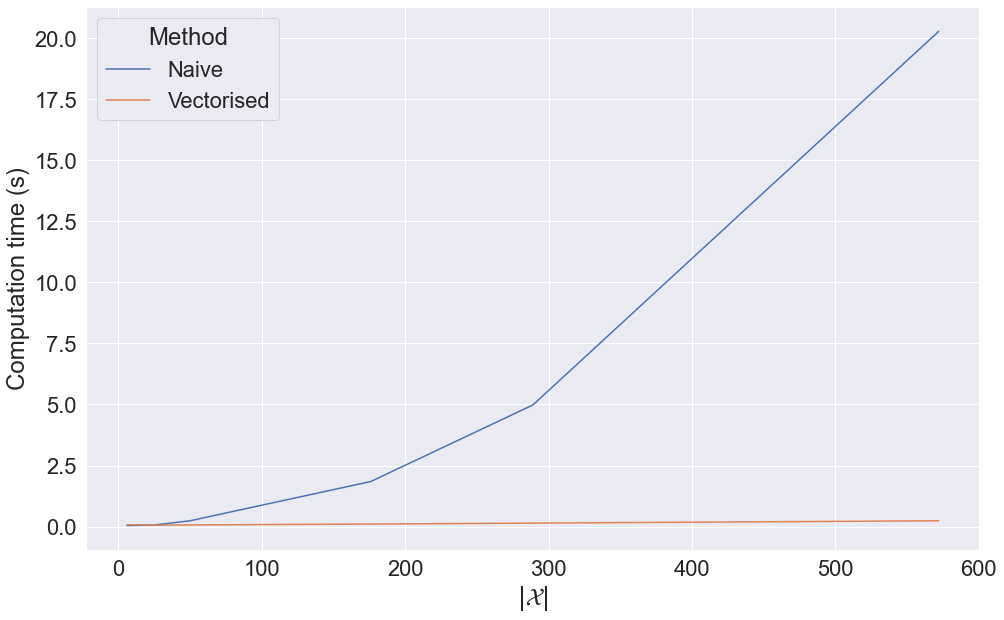
\includegraphics[width=\textwidth]{imp_utau}
	\caption{A illustration for the computer time taken to calculate $\Sigma_\mathcal{X}$ for the naive and vectorised methods for multiple sizes of observed data. Here we use $K = 5$ for our illustrative example. The above computation times were taken from a single machine running with the Darwin kernel Version 21.1.0 on an i386 processor with 16Gb of RAM.}
	\label{fig:imp_utau}
\end{figure}

This method for calculation of $\Sigma_{\mathcal{X}}$ has an additional use in the calculation of the log marginal likelihood, given in Equation~\ref{eqn:mll_cpace}.
Renowned for being the bottle neck of a standard Gaussian process model, \citep{williams_gaussian_2006}, the minimisation of the log marginal likelihood is typically time consuming due to the need to calculate the inverse and determinant of the covariance matrix of the process for the training observations.
This can be particularly challenging since the standard approach for doing so involves the cholesky decomposition of $\ve{\Sigma}\left( \ve{Y}, \ve{Y} \right)$.
The algorithm used to compute this cholesky decomposition has computational complexity of $O(\frac{\lvert \mathcal{X} \rvert^3}{6})$.
This doesn't scale particularly well as $\lvert \mathcal{X} \rvert$ gets larger.
However, we can use the structure of $\Sigma_{\mathcal{X}}$ to improve this in our CPACE model.

In particular, noting that $\ve{\Sigma}\left( \ve{Y}, \ve{Y} \right) = \Sigma_\mathcal{X} + \sigma_\varepsilon^2 \ve{I}$ has a very particular structure.
Namely; 
\begin{equation}
	\ve{\Sigma}\left( \ve{Y}, \ve{Y} \right) = \ve{U} \ve{A} \vesup{U}{\transpose} + \sigma_\varepsilon^2 \ve{I}
\end{equation}
We can use the Woodbury matrix identity to calculate it's inverse, and the matrix determinant lemma to calculate its determinant.

The Woodbury matrix identity, \citep{woodbury_inverting_1950}, named after \citeauthor{woodbury_inverting_1950}, states that inversion of a rank $k$ matrix can be computed by applying a rank $k$ correction to the inverse of the original matrix.
In our model we have:
\begin{equation}
	 \left( \ve{U} \ve{A}  \vesup{U}{\transpose} + \sigma_\varepsilon^2 \ve{I} \right)^{-1} = p \ve{I} - p \ve{U}\left(\vesup{A}{-1} + p^2\vesup{U}{\transpose}\ve{U}\right)^{-1} \vesup{U}{\transpose}
	 \label{eqn:woodbury}
\end{equation}
where $p = \frac{1}{\sigma_\varepsilon^2}$ is the precision.
Here this has reduced the large $\lvert \mathcal{X} \rvert \times \lvert \mathcal{X} \rvert$ matrix inversion into two smaller inversions of size $(K\times N) \times (K \times N)$.
We note now that the inversion of the matrix $\ve{A}$ can be simplified further due to its block diagonal structure.
This inversion actually only requires $K$ lots of $N \times N$ inversions.
The outer inversion, $\left(\vesup{A}{-1} + p^2\vesup{U}{\transpose}\ve{U}\right)$ isn't inverted directly as for the marginal log likelihood we require $\ve{\Sigma}\left( \ve{Y}, \ve{Y} \right)^{-1} \ve{Y}$.
Hence by postmultiplying Equation~\ref{eqn:woodbury} by $\ve{Y}$ we can use the cholesky factor of this outer matrix and a cholesky solve against $\vesup{U}{\transpose}\ve{Y}$ to calculate this component in a numerical stable way.

For the marginal log likelihood we also require the determinant of $\ve{\Sigma}\left( \ve{Y}, \ve{Y} \right)$.
The matrix determinant lemma, \citep{harville_determinants_1997}, is the analogue to the Woodbury matrix identity for their determinants.
By using the matrix determinant lemma the determinant of $\ve{\Sigma}\left( \ve{Y}, \ve{Y} \right)$ can be found as: 

\begin{equation}
	\det \left(\ve{\Sigma}\left( \ve{Y}, \ve{Y} \right) \right) = \det \left(\vesup{A}{-1} + p^2\vesup{U}{\transpose}\ve{U}\right) \det (\ve{A}) \det (\sigma_\varepsilon^2 \ve{I})
\end{equation}

Again, this works in tandem with the cholesky decomposition of the larger outer matrix and if the inner inversion of $\ve{A}$ is also calculated with a cholesky decomposition the full determinant follows easily from the Woodbury inversion in Equation~\ref{eqn:woodbury}.

The use of these formulas isn't an approximation, and thus we retain the exact properties of the Gaussian process if we follow the above implementation whilst reducing the complexity of calculating the expensive operations in the marginal log likelihood from $O(\frac{\lvert \mathcal{X} \rvert^3}{6})$ to $O((KN)^3)$.
This essentially means that the number of time points we observe at each spatial location is not a limiting factor in our estimation procedure.
Since our computation time only has cubic growth with the number of spatial points and model components.
Figure~\ref{fig:imp_woodbury} highlights the effect of using the above method on computation time for a matrix inversion. 
As can be seen from this the above implementation using the Woodbury inversion technique reduces the computational burden significantly.

\begin{figure}
	\centering
	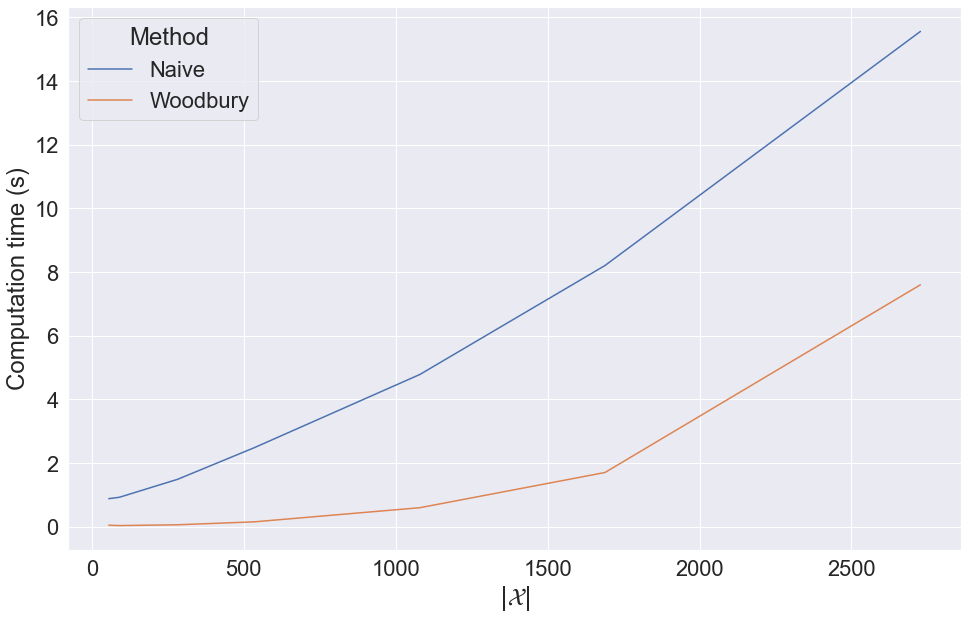
\includegraphics[width=\textwidth]{imp_woodbury}
	\caption{An illustration for the computer time taken to calculate $\Sigma_\mathcal{X}$  inverse for the naive and vectorised methods for multiple sizes of observed data. This illustrative example uses $K=5$ number of components in the CPACE model. The above times were taken from a single machine running with Darwin kernel Version 21.1.0 on an i386 processor with 16Gb of RAM.}
	\label{fig:imp_woodbury}
\end{figure}

The above implementation for our CPACE model makes the model feasible on relatively large data sets.
However, it still requires multiple evaluations of the marginal log likelihood to estimate the hyper parameters of the spatial kernels.
We discuss our approach to this in the following section, Section~\ref{ssec:imp_gp_min}.

\subsection{Maximising the Marginal Log Likelihood \label{ssec:imp_gp_min}}
We have stated in Chapter~\ref{cha:cpace} that any hyper parameters of the CPACE model, most prominently the spatial kernel hyper parameters, are estimated by minimising the negative log marginal likelihood of the model; this is equivalent to maximising the marginal log likelihood.
To do so we follow our minimisation methodology from Section~\ref{sec:psplines} and use a gradient descent based algorithm.
In particular, we also use automatic differentiation to calculate our gradients.
This is discussed in Section~\ref{sec:auto_diff}.

In our implementation, we have opted to use a stochastic gradient descent (SGD), \citep{sra_optimization_2012}, algorithm for this.
Whilst in principle any gradient descent algorithm should perform fine, we found through experimentation that a SGD algorithm tended to perform best.
Our intuitive reasoning for this is that due to the large number of hyper parameters in the CPACE framework, it is relatively easy for the gradient descent algorithms to get stuck in local optima.
The stochastic nature of SGD essentially randomly perturbs the true direction of travel by approximating the gradient from a random subset of data. 
This added variability gives it the chance to overcome any small local optima caused by specific hyper parameters, whereas deterministic approached like N-ADAM, \citep{dozat_incorporating_2016}, tended not to find these.

Two more items are important in implementing such a gradient descent approach to maximising the marginal log likelihood; the initialisation of the algorithm and the stopping criterion.
To initialise our minimisation routine we opt for random starts.
In particular, we pick a number of places from the likely domain of the hyper parameters.
For each choice we calculate the marginal log likelihood, then start the SGD initialised at the point which has maximum marginal log likelihood.
Whilst this doesn't guarantee to aide in finding global optima it is a often used heuristic, \citep{sra_optimization_2012}.
The reasoning being it gives the descent algorithm a chance of starting in a location where the global optimum may exist.
The exact number of initialisation attempts is chosen by the user and is usually problem dependent. 
For example; in our simulation study, Chapter~\ref{cha:application},  we use $32$ random initialisations.
The trade off for choosing this is purely down to time available for training.
There is a similar trade off used in deciding when to stop the gradient descent algorithm.

As with any minimisation procedure, how to stop is often a tricky problem.
For SGD it is of particular importance as the stochastic nature may mean you can step away from the gradient only to return to it later in the routine.
Early stopping is a classic heuristic to prevent wasted computation when this happens, \citep{sra_optimization_2012}.
In our implementation for our simulation study we decided to stop when the absolute relative change in gradient was less than a tolerance of $0.001$\% or the relative change of the maximum log likelihood was less than a tolerance of $1e^{-5}$\%. 
Again, these stopping criterion are usually problem dependent, \citep{sra_optimization_2012}.
The larger tolerance for stopping can often reduce estimation time but may mean you end up with sub-optimal hyper parameters.
A narrow tolerance may mean you produce more optimal hyper parameter estimation, but can cause the computational time to increase largely.

Finally, to help speed up computation of this minimisation procedure we implement batched stochastic gradient descent, \citep{li_efficient_2014}.
We consider our training datasets in batches, and perform the update for the hyper parameters on each batch in sequence.
Our training data is split into $b$ sized batches, $b$ is chosen heuristically.
Typical choices are $16, 32$, and $64$.
A single iteration, or epoch, of estimation of our hyper parameters results in batching our training data then looping through all batches of our training data and performing a SGD update step.
This effectively add two improvements to our estimation procedure.
There is a dramatic speed up since now gradients of the marginal log likelihood are computed over the batch, so the batch size, $b$, is determining our maximum size of the computationally complex cholesky decomposition as described in Section~\ref{ssec:imp_gp_min}.
We note that when we split our training data up into batches, we split entirely on the location, thus we are splitting $N$ into batches.
This means that all temporal observations for a particular functional data are contained in the same batch.

This batched approach to estimating kernel hyper parameters is well used in Machine learning, \citep{li_efficient_2014}. 
The speed up of computation offered by this is then hampered by an added noisy updated to our hyper parameters from the SGD update over a single batch.
In practice, this approach works well with SGD and is widely used, \citep{li_efficient_2014}, \citep{sra_optimization_2012}.

In this section we have detailed our estimation procedure for the hyper parameters in the CPACE framework.
As with most Gaussian process implementation we estimate these through maximising the marginal log likelihood.
We have detailed our implementation of this maximisation approach using a batched gradient descent algorithm. 
What remains to be specified is how we obtain the gradients with respect to the hyper parameters which are used in such gradient based algorithms.
We do so in the following section.

\section{Automatic Differentiation \label{sec:auto_diff}}
In our CPACE framework, described in Chapter\ref{cha:cpace}, there a two main places where we need to estimate hyper parameters.
In the estimation of eigen functions through penalised B-Spline smoothing and in the estimation of our spatial kernel hyper parameters.
We have outlined our implementation of estimating these in Sections~\ref{sec:psplines}, \ref{ssec:imp_gp_min} respectively.
Each of which requires a gradient based optimiser, and thus need gradients with respect to hyper parameters.
In this section we outline how we go about obtaining these.

There are three popular methods for computing gradients and Hessians of complex mathematical functions using a computer; numeric, symbolic, and automatic differentiation.
Numeric differentiation uses the method of finite differences to approximate the derivative.
It can introduce rounding errors through the discretization of the problem as well as issues surrounding cancellation causing the gradient to be a poor approximation of the exact gradient.
Symbolic differentiation manipulates expression through mathematics, using known gradients of simple operations and a combination of the product and chain rules of derivatives.
These are then combined to a single expression which represents the gradient of the function which is then evaluated at locations of interest.
It is often inappropriate to use since converting computer code into a single mathematical expression of the gradient it often difficult, especially if there are conditions such as if and else statements. 
This can lead to inefficient code, \citep{baydin_automatic_2018}.

Automatic differentiation is a series of techniques that allows one to efficiently and accurately evaluate derivatives of numeric functions expressed as computer programs, \citep{neidinger_introduction_2010}.
It exploits the fact that a computer program executes a series of elementary mathematical operations and functions.
It is broadly split into two categories; forward mode and reverse mode.
We discuss reverse mode automatic differentiation briefly as it is the implementation we use in this work.
For more detailed discussion on these approaches we refer the reader to \citep{neidinger_introduction_2010}.

Reverse mode automatic differentiation; calculates the (partial) derivative(s) at a point by using a forward and reverse pass through the elementary functions.
We give a simple example to illustrate.

Suppose we wish to evaluate the partial derivatives of:
\begin{equation}
	z = x_1 x_2 + cos(x_1)
\end{equation}
with respect to $x_1$ and $x_2$ at $x_1=3$, $x_2=4$.
Automatic differentiation begins by breaking this up into our component functions; exactly as a computer program would. 
\begin{eqnarray*}
	w_1 &=& x_1 \\
	w_2 &=& x_2 \\
	w_3 &=& w_1 w_2 \\
	w_4 &=& \cos\left(w_1\right) \\
	w_5 &=& w_3 + w_4 \\
	z &=& w_5
\end{eqnarray*}

The forward pass then simply evaluates these components at $x_1=3$ and $x_2=4$ and saving the results.
That is: 
\begin{eqnarray*}
	w_1 &=& x_1 = 3 \\
	w_2 &=& x_2 = 4\\
	w_3 &=& w_1 w_2 = 12 \\
	w_4 &=& \cos\left(w_1\right) = -0.99 \\
	w_5 &=& w_3 + w_4  = 11.01\\
	z &=& w_5 = 11.01
\end{eqnarray*}

The backward pass then starts at the last node and evaluates the derivative with respect to its parent components.
So firstly, $\frac{dz}{dw_5} = 1$.
Then next, $w_5$ depends linearly on $w_3$ and $w_4$, so we calculate the derivative of $w_5$ with respect to these; then can use the chain rule to accumulate this up to the derivative of $z$ with respect to these components, keeping each. 
That is:
\begin{eqnarray*}
	\frac{dz}{dw_3} &=& \frac{dz}{dw_5}\frac{dw_5}{dw_3} = 1 \times 1 \\
	\frac{dz}{dw_4} &=& \frac{dz}{dw_5}\frac{dw_5}{dw_4} = 1 \times 1
\end{eqnarray*}

We can continue on in this fashion.
Then $\frac{dz}{dw_2} = \frac{dz}{dw_3}\frac{dw_3}{dw_2} = w_1 = 2$ as we know $w_1$ from our forward pass.
Similarly $\frac{dz}{dw_1} = \frac{dz}{dw_3}\frac{dw_3}{dw_1} +  \frac{dz}{dw_4}\frac{dw_4}{dw_1}= w_2 - \sin(w_1)= 4 - \sin(3)$.
Evaluating this gives our partial derivates:
\begin{eqnarray*}
	\frac{dz}{dx_1} &=& 2 \\
	\frac{dz}{dx_2} &=& 4 - \sin(3)
\end{eqnarray*}

This procedure is essentially creating a graph of relatively simple computations, of which shared results can be utilised.
Software is readily available which deals with the creating, storing, and efficient evaluation of such graphs.
For example, the \verb*|tensorflow| library, \citep{abadi_tensorflow_2016}.

The above illustration is easily extended to multivariate functions and can handle high number of partial derivatives, \citep{neidinger_introduction_2010}.
This is because we can compute all partial derivative that we are interested in a single flow through both the forward and reverse path.
As long as we have a few components with known derivatives, such as $\sin, \cos, \exp, \dots$, we can then quickly evaluate derivatives of complex functions with respect to many parameters.
This methodology doesn't suffer particularly from round off error due to never subtracting similar numbers, unlike in finite difference approaches which is the basis for the method.

In our implementation of the CPACE framework we make use of reverse mode automatic differentiation.
We use the Python package, \verb*|tensorflow| which is capable of calculating gradients through this exact approach, \citep{abadi_tensorflow_2016}. 
This mean our gradient based optimisation procedures for penalised B-spline smoothing and spatial kernel hyper parameters can be achieved, even when the number of parameters we need derivatives for is extremely high such as the case for the Gibbs kernel.
We discuss this particular kernel more in the following section.


\section{Gibbs Kernel \label{sec:gibbs_kernel}}
This Gibbs kernel is our main non-stationary kernel of interest in both our simulation study and application to the CESM-LE study; Chapters~\ref{cha:application}`~\ref{cha:real_application} respectively.
The general form of which , previously discussed in Section~\ref{sec:gibbs_kernel} and given here for convenience is: 
\begin{equation}
	k\left(s_{i}, s_{j}\right) = \sum_{q=1}^{Q} \sqrt{\frac{2l_q(s_i)l_q(s_j)}{l_q(s_i)^2 + l_q(s_j)^2}} \exp \left(-\frac{\left(s_i - s_j\right)^2}{l_q(s_i)^2 + l_q(s_j)^2}\right)
\end{equation}
where $s_i, s_j$ are the points of evaluation, $Q$ is the number of components in the kernel and $l_q$ is the length scale  function for component $q$.
In this section we discuss the implementation of the length scale model, $l_q$ for $q=1,2,\dots,Q$ that we use for the simulation and CESM-LE study.

We mentioned briefly in Sections~\ref{sec:sim_study},~\ref{sec:cesm_kernels} that we use a Neural network model for the length scale, $l_q$.
This is not the only model that could be used.
For example, \citep{paciorek_spatial_2006} considers parametrising their length scale models using a latent Gaussian process.
In our implementation of the Gibbs kernel, we have opted to use a Neural network model for a couple of reasons.
Firstly; given a sufficient structure they are flexible and can approximate a variety of surfaces.
Secondly; they are somewhat agnostic to specific construction.
That is as long as the network structure we use is sufficiently large, we can be somewhat lazy about exact network structure. 
That isn't to say we should be lazy in constructing these hyper parameter models, but that given they are not our main area of interest in the CPACE framework, we should be happy that we can give a general construction which should perform reasonably well.
Finally, they are fast to evaluate and fast to train, \citep{abadi_tensorflow_2016}.
In particular, such a network model fits in naturally to the use of \verb*|tensorflow| to implement the CPACE framework.

Having decided on a structure of the Neural network, for example in our simulation study we used a model with two hidden layers each containing $32$ neurons using the ReLu activation function, there is still the practical consideration to ensure the length scale model it represents is positive.
The simplest way to do this is to model the log length scale using the neural network and exponentiate the output.
This is how we have implemented the Gibbs kernel in both the simulation study and application to the CESM-LE dataset. 

Estimation of the parameters of the length scale model follows as in Section~\ref{sec:cpace_gp} where they are estimated in conjunction with the other hyper parameters of the CPACE framework.
This is where having an efficient and fast calculation of the log marginal likelihood and its gradient with respect to the hyper parameters become powerful.
Since without this using a length scale model which relies on a large number of hyper parameters would be infeasible in terms of computational cost.

Finally, we give an indicative example of the output from an estimated length scale model using the above approach in Figure~\ref{fig:gibbs_lengthscale}.
This is taken from a single simulation for the pressure variable from the CESM-LE dataset.
The full model results given in Section~\ref{ssec:cesm_ps}.
We use this to highlight that the Neural network approach gives a reasonable method for implementing the Gibbs kernel in the CPACE framework.
As we can see it captures interesting variation in the length scale which corresponds to distinct areas of the globe where pressure often has differing correlation structure.


Whilst we haven't attempted to show that using such a Neural network model is the definitive way to implement the length scale models in the Gibbs kernel; through our simulation studies and application to CESM-LE dataset this approach has faired well.
It often converges to reasonably interpretable structures and the results for the CPACE models utilising this implementation were comparable to those that used a more standard kernel.

\begin{figure}
	\centering
	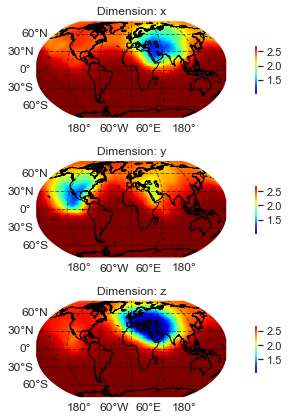
\includegraphics[width=\textwidth]{gibbs_lengthscale}
	\caption{An indicative example of the length scale model used in our implementation of the Gibbs kernel. The full length scale model for each dimension of the data set is plotted in the corresponding graphs. Here we show the first component of the Gibbs kernel only and for a single spatial kernel of the CPACE framework. We use this to highlight the reconstructive ability of a relative simple Neural network model for representing the full unknown length scale model used in the Gibbs kernel..}
	\label{fig:gibbs_lengthscale}
\end{figure}